\chapter{Results}

This chapter presents and analyzes the results obtained using the methodology
presented in the previous chapter.

\section{Performance Results}

Using software-only hashing produced the results in table \ref{tab:Perf-SW}. As can be seen
in the plot in figure \ref{fig:sw-scaling} adding more processors after the third produces no
additional performance gain.\todo{We'll rotate this table or maybe move it to an appendix?}

The reason for this is that all cores must make frequent accesses to DRAM, which causes the
DRAM tile to quickly become congested.

Another interesting effect to note in the results is how the XY routing affects the performance
of each tile. The more tiles that tries to access main memory through a tile, the less
performance that tile has; it seems that SHMACs router system favours requests originating
from other tiles before requests originating from the tile itself.

\begin{table}
\tiny
\begin{tabular}{| l || r | r | r | r | r | r | r | r | r | r | r | r | r | r | r | r |}
  \hline 
  \textbf{Sum} [H/s] & \textbf{0} & \textbf{1} & \textbf{2} & \textbf{3} & \textbf{4} & \textbf{5} & \textbf{6} & \textbf{7} & \textbf{8} & \textbf{9} & \textbf{10} & \textbf{11} & \textbf{12} & \textbf{13} & \textbf{14} & \textbf{15}   \\
  \hline                       
  \textbf{13041} & 13041 & - & - & - & - & - & - & - & - & - & - & - & - & - & - & - \\
  \textbf{26105} & 13041 & 13064 & - & - & - & - & - & - & - & - & - & - & - & - & - & - \\
  \textbf{39185} & 13041 & 13064 & 13080 & - & - & - & - & - & - & - & - & - & - & - & - & - \\
  \textbf{36470} & 11114 & 10801 & 7258 & 7297 & - & - & - & - & - & - & - & - & - & - & - & - \\
  \textbf{36449} & 8064 & 8033 & 4065 & 4063 & 12224 & - & - & - & - & - & - & - & - & - & - & - \\
  \textbf{36452} & 6063 & 6073 & 3047 & 3047 & 9140 & 9082 & - & - & - & - & - & - & - & - & - & - \\
  \textbf{36450} & 4237 & 4244 & 2125 & 2125 & 6367 & 6367 & 10985 & - & - & - & - & - & - & - & -\\
  \textbf{36457} & 4044 & 4051 & 2027 & 2027 & 6077 & 6077 & 6077 & 6077 & - & - & - & - & - & - & - \\
  \textbf{36446} & 2686 & 2691 & 1345 & 1345 & 4035 & 4035 & 4035 & 4035 & 12239 & - & - & - & - & - & - & -\\
  \textbf{36457} & 2022 & 2026 & 1013 & 1013 & 3039 & 3039 & 3039 & 3039 & 9131 & 9096 & - & - & - & - & - & -\\
  \textbf{37640} & 1463 & 1467 & 733 & 733 & 2200 & 2200 & 2200 & 2200 & 6600 & 6600 & 11244 & - & - & - & - & -\\
  \textbf{36442} & 1017 & 1021 & 511 & 511 & 1531 & 1531 & 1531 & 1531 & 4595 & 4595 & 9188 & 8880 & - & - & - & -\\
  \textbf{36868} & 1020 & 1035 & 517 & 517 & 1550 & 1550 & 1550 & 1550 & 4656 & 4656 & 9161 & 4553 & 4553 & - & - & -\\
  \textbf{36447} & 1012 & 1016 & 508 & 508 & 1525 & 1525 & 1525 & 1525 & 4573 & 4573 & 9146 & 2266 & 2266 & 4479 & - & -\\
  \textbf{36444} & 1010 & 1014 & 507 & 507 & 1521 & 1521 & 1521 & 1521 & 4564 & 4564 & 9128 & 1524 & 1524 & 3031 & 2987 & -\\
  \textbf{37645} & 1042 & 1046 & 523 & 523 & 1569 & 1569 & 1569 & 1569 & 4706 & 4706 & 9411 & 1572 & 1572 & 3124 & 1572 & 1572\\
  \hline  
\end{tabular}
\caption{Software hash results, using varying numbers of cores}
\label{tab:Perf-SW}
\end{table}

\begin{figure}
	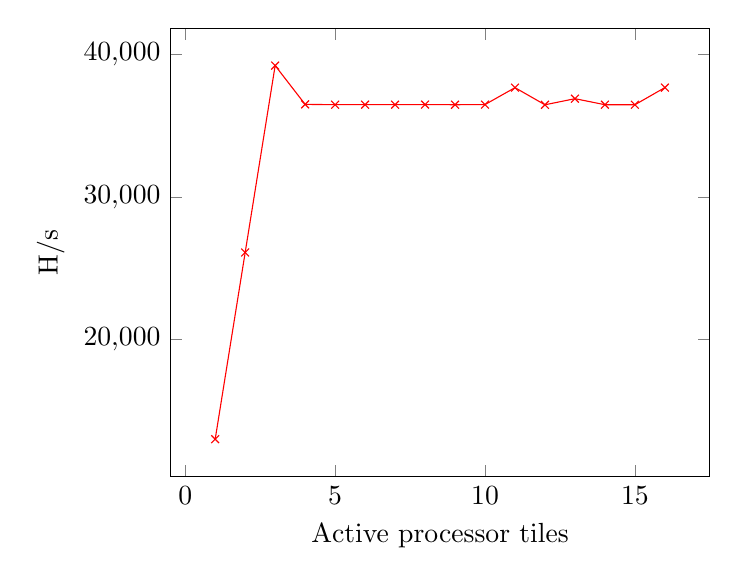
\begin{tikzpicture}
		\begin{axis}[
			xlabel=Active processor tiles,
			ylabel=H/s,
			scaled ticks=false]
		\addplot[color=red,mark=x] coordinates {
			(1, 13041)
			(2, 26105)
			(3, 39185)
			(4, 36470)
			(5, 36449)
			(6, 36452)
			(7, 36450)
			(8, 36457)
			(9, 36446)
			(10, 36457)
			(11, 37640)
			(12, 36442)
			(13, 36868)
			(14, 36447)
			(15, 36444)
			(16, 37645)
		};
		\end{axis}
	\end{tikzpicture}
	\caption{Scaling using software hashing}
	\label{fig:sw-scaling}
\end{figure}


\begin{table}
\begin{tabular}{ | l || r | r | r | r |}
  \hline 
  \textbf{SUM \textbackslash T ID} & \textbf{0} & \textbf{1} & \textbf{2} & \textbf{3}\\
  \hline                       
  \textbf{37711} & 37711 & - & - & - \\
  \textbf{80237} & 37655 & 42582 & - & - \\
  \textbf{117791} & 37556 & 42450 & 37785 & - \\
  \textbf{150799} & 37391 & 42271 & 37496 & 33641 \\
  \hline  
\end{tabular}
\caption{Hashing per second, using the SHA256-hashing module. Only up to 4 processors worked}
\label{tab:Perf-SHA}
\end{table}

\begin{table}
\begin{tabular}{| l || r | r | r | r |}
  \hline 
  \textbf{SUM \textbackslash T ID} & \textbf{0} & \textbf{1} & \textbf{2} & \textbf{3}\\
  \hline                       
  \textbf{42209} & 42209 & - & - & - \\
  \textbf{86979} & 41787 & 45192 & - & - \\
  \textbf{126705} & 41097 & 44456 & 41152 & - \\
  \textbf{159372} & 39799 & 43303 & 39824 & 36446 \\
  \hline  
\end{tabular}
\caption{Hashing per second, using the SHA256-hashing module and DMA module. Only up to 4 processors worked}
\label{tab:Perf-SHADMA}
\end{table}

\begin{figure}
	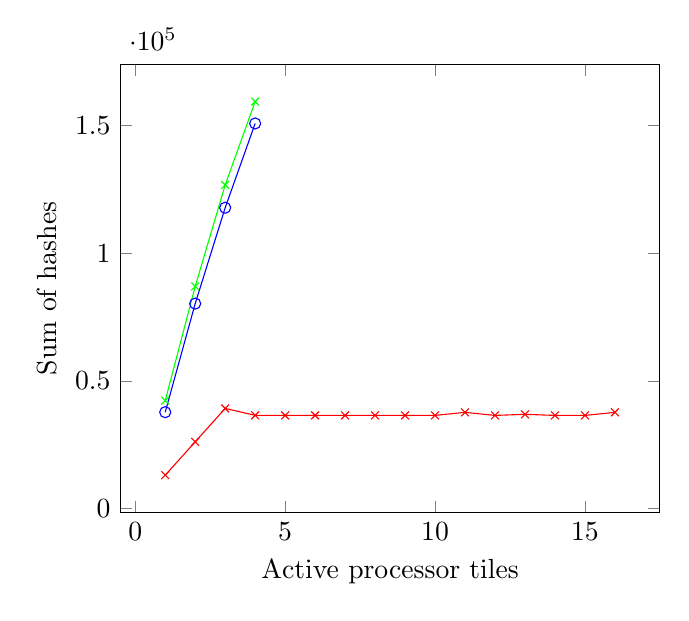
\begin{tikzpicture}
		\begin{axis}[
			xlabel=Active processor tiles,
			ylabel=Sum of hashes]
		\addplot[color=red,mark=x] coordinates {
			(1, 13041)
			(2, 26105)
			(3, 39185)
			(4, 36470)
			(5, 36449)
			(6, 36452)
			(7, 36450)
			(8, 36457)
			(9, 36446)
			(10, 36457)
			(11, 37640)
			(12, 36442)
			(13, 36868)
			(14, 36447)
			(15, 36444)
			(16, 37645)
		};
		\addplot[color=blue,mark=o] coordinates {
			(1, 37711)
			(2, 80237)
			(3, 117791)
			(4, 150799)
		};
		\addplot[color=green,mark=x] coordinates {
			(1, 42209)
			(2, 86979)
			(3, 126705)
			(4, 159372)
		};
		\end{axis}
	\end{tikzpicture}
	%\caption{Sum of hases per second}
	%\label{fig:Perf-plot}
\end{figure}

\section{Power and energy efficiency}

We must measure the power from the wall, before we can add anything here.












